\documentclass{article}
\usepackage{tikz}
\usepackage{xcolor}

\begin{document}
\pagestyle{empty}

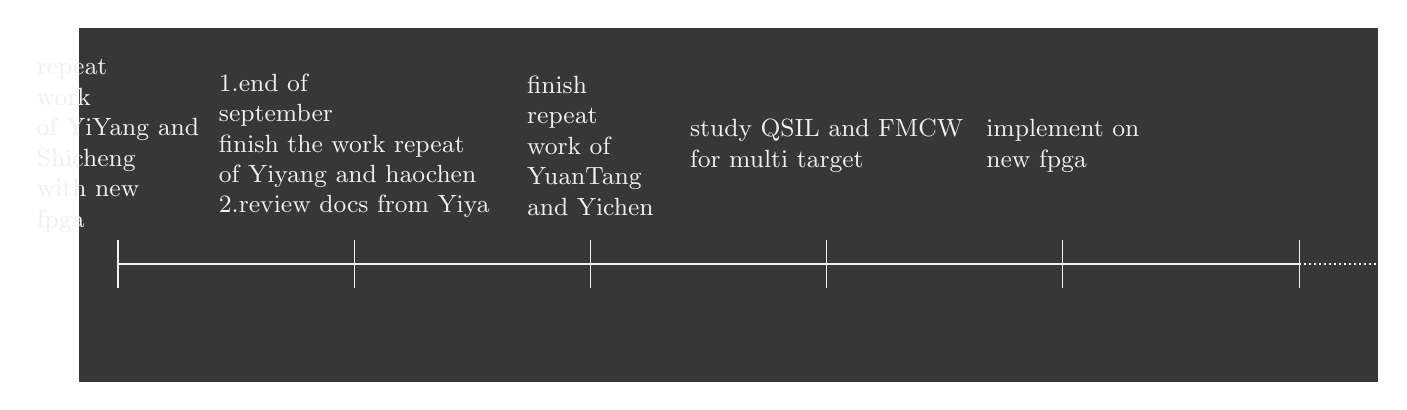
\begin{tikzpicture}
% Define colors
\definecolor{darkbg}{RGB}{55,55,55}
\definecolor{lighttext}{RGB}{240,240,240}

% Set background
\fill[darkbg] (-0.5,-1.5) rectangle (16,3);

% Main timeline
\draw[lighttext, thick] (0,0) -- (15,0);

% Timeline vertical markers
\draw[lighttext] (0,-0.3) -- (0,0.3);
\draw[lighttext] (3,-0.3) -- (3,0.3);
\draw[lighttext] (6,-0.3) -- (6,0.3);
\draw[lighttext] (9,-0.3) -- (9,0.3);
\draw[lighttext] (12,-0.3) -- (12,0.3);
\draw[lighttext] (15,-0.3) -- (15,0.3);

% Dotted line extension
\draw[lighttext, densely dotted, thick] (15,0) -- (16,0);

% Timeline labels positioned above the line
\node[lighttext, align=left, font=\small] at (0,1.5) {repeat\\work\\of YiYang and\\Shicheng\\with new\\fpga};

\node[lighttext, align=left, font=\small] at (3,1.5) {1.end of\\september\\finish the work repeat\\of Yiyang and haochen\\2.review docs from Yiya};

\node[lighttext, align=left, font=\small] at (6,1.5) {finish\\repeat\\work of\\YuanTang\\and Yichen};

\node[lighttext, align=left, font=\small] at (9,1.5) {study QSIL and FMCW\\for multi target};

\node[lighttext, align=left, font=\small] at (12,1.5) {implement on\\new fpga};

\end{tikzpicture}

\end{document}